\documentclass[11pt,a4paper,oneside, openright]{article}
\usepackage{graphicx}
\usepackage[british]{babel}
\usepackage[utf8]{inputenc}
\usepackage{mathtools}
\usepackage{setspace}
\usepackage{verbatim}
\usepackage{tikz}
\usetikzlibrary{trees}
\usepackage{url}

\begin{document}
{\setstretch{1.0}
  \begin{titlepage}
  	\centering
  	
\includegraphics[width=6cm]{images/unipi.eps}\par
  	\vspace{1.5cm}
  	{\huge\textsc{Performance evaluation of a CRAN system}\par}
  	\vspace{2cm}
  	Gerardo \textsc{Alvaro}\par
  	Francesco \textsc{Barbarulo}\par
    Francesco \textsc{Fornaini}

  	\vfill

    % Bottom of the page
  	{\large 2018-2019\par}
  \end{titlepage}
}


\tableofcontents

\newpage

\section{Introduction}
The system examined is a simplified version of an architecture presented for future cellular networks, called Cloud-RAN (CRAN).

\subsection{Description of the system}
 At the center of this system there is a central processing unit (BBU), which is responsible for forwarding the packets received from an Application Server (AS) to one of the N remote radios (RRH) connected to it. Each RRH serves a single cell, and each packet generated by the AS has one of these cells as a destination, taken uniformly from those available. Each data packet has a size $s$ and a new one is generated every $t$ seconds. The BBU has an interface to each of the RRHs and communicates with only one of them at a time, at a speed of X bytes/s. If the BBU interface with the RRHs is busy, the data packets are queued and served using the FIFO policy.

When the BBU receives a packet from the AS, it can operate in two different ways:
\begin{itemize}
	\item[A)]It retransmits directly the packet to the RRH which serves the destination cell N;
	\item[B)]The BBU compress the packet, reducing its size by C\% and retransmitting it to the proper RRH. Once arrived at the RRH, the packet is decompressed. Such operation takes S seconds, where S is given by $ S = C \cdot 50ms $. Only one packet can be decompressed at a time. If the decompressing process is busy, the incoming data packets are queued and served using a FIFO policy.
\end{itemize}

Packet size and interarrivals are random variables described as:
\begin{itemize}
	\item exponential distribution of $t$;
	\item exponential and lognormal distribution of $s$.
\end{itemize}

\subsection{Objectives and performance indexes}
The objective of the study is to determine if and under what conditions it is better to perform packet compression or not, or possibly to adopt a hybrid mode of operation.
For a correct evaluation of the system will be taken as reference the mean end-to-end delay of packets.

\section{Model}
Before introducing the model, we make some semplifications which do not affect the final results.
\subsection{Assumptions}
First of all we make some assuptions:
\begin{itemize}
    \item Propagation times ($ T_{prop} $) are negligible;
    \item In case A, the end-to-end delay is computed when the packet arrives at the RRH;
    \item In case B, the end-to-end delay is computed until the packet decompression is finished;
    \item BBU switching time (time needed to change the output gate) is negligible;
    \item In case B, the compression time on BBU is negligible;
    \item Packets are not corrupted;
    \item No packet loss at the buffers (infinite buffers).
\end{itemize}

With these assumptions, we can compute the end-to-end delay as following:

$$ T_{delay} =  T_{waiting\_bbu} + T_{transmission} + T_{waiting\_rrh} + T_{decompression} $$

where 

$$ T_{transmission} = \frac{1}{\mu_{bbu}} = \frac{s}{X} $$

and

$$ T_{decompression} = \frac{1}{\mu_{rrh}} = C \cdot 50ms $$

\subsection{Validation}
The simulator has been validated through a comparison with a queueing theory model of the system.

The system has been modelled as an Open Jackson Network because all the hypotheses are verified since external arrivals are poissonian and routing probabilities are state-independent because they are uniform as specified in the requirements.

\begin{figure}[h]
    \centering
    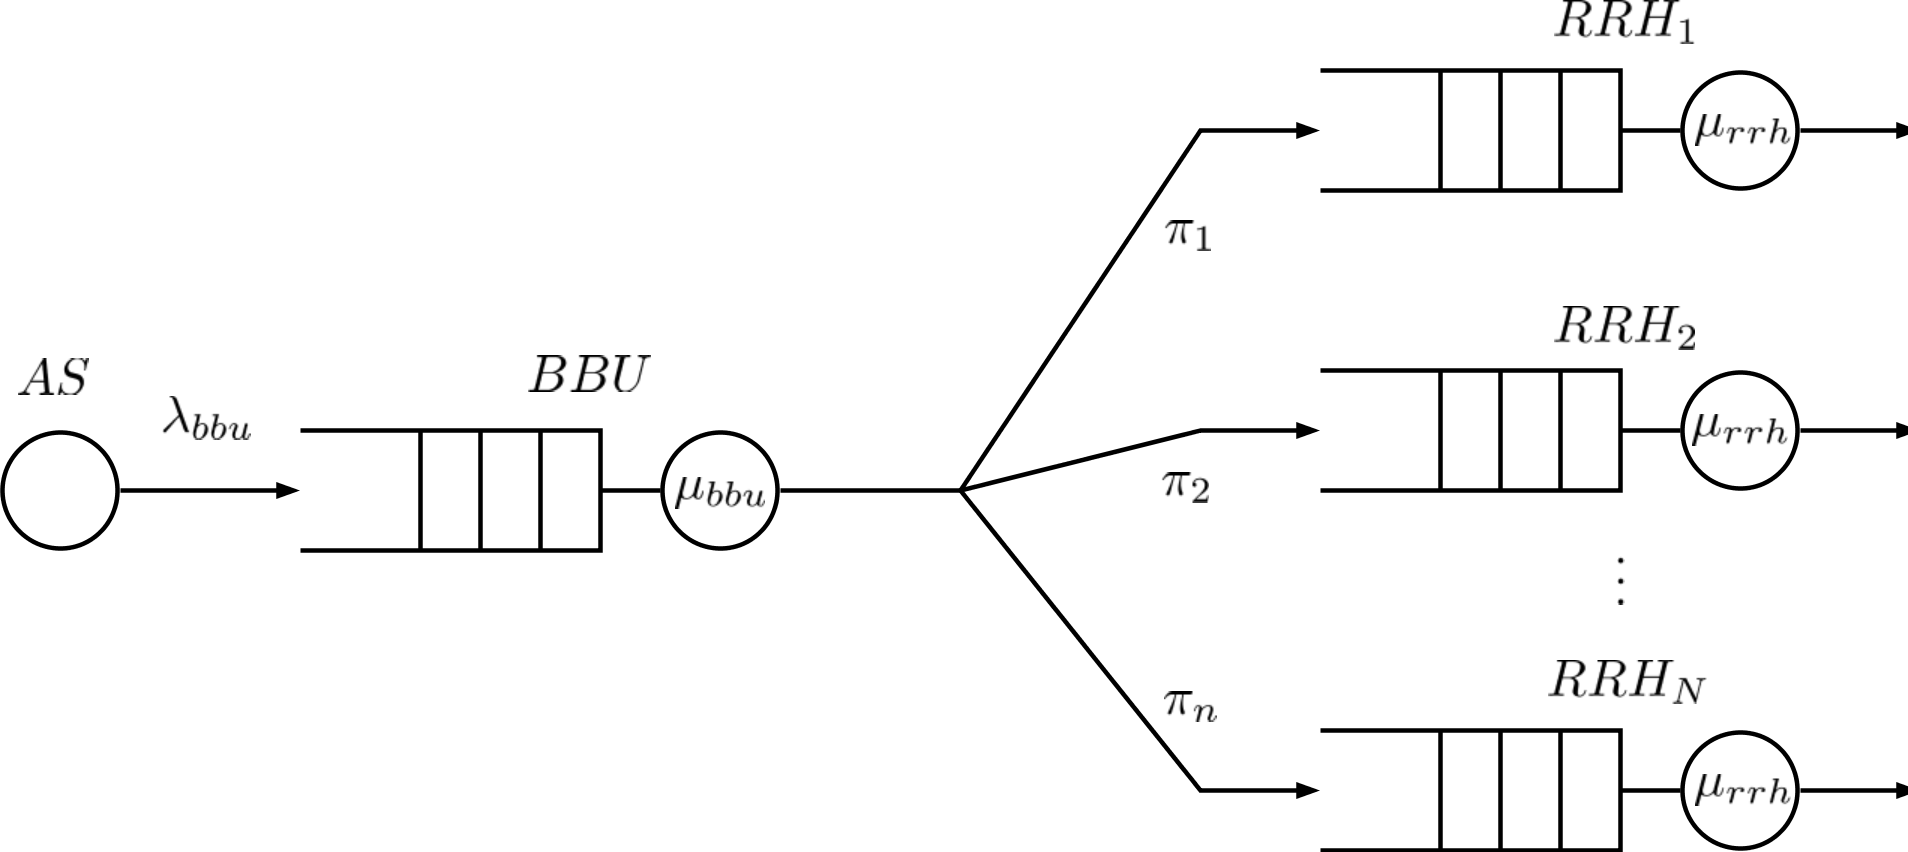
\includegraphics[width=0.9\textwidth]{images/model}
    \caption{Queuing network model}
    \label{fig:model}
\end{figure}

\subsubsection{Stability conditions}
In order to compute the stabilty conditions we have to distinguish between the two cases.

In case A we have to respect only one condition regarding the BBU. Indeed, on the RRHs we will never have queues because when the packet arrives, it is immediately consumed.
Hence, the stability condition is the following:

$$ \lambda_{bbu} < \mu_{bbu}, \quad \lambda_{bbu} = \frac{1}{t}, \quad \mu_{bbu} = \frac{X}{s}$$

\begin{equation} \label{eq:rho-bbu}
\rho_{bbu} = \frac{\lambda_{bbu}}{\mu_{bbu}} = \frac{s}{t \cdot X} < 1
\end{equation}

Note that $s$ represents the number of bytes that the BBU has to transmit. From now on we will consider:
$$s = s\cdot(1-\frac{C}{100})$$

In case B we have also to take in account the stability condition on the RRHs because now the RRH service time is not null and depends on the compression percentage. Furthermore the arrival rate to each RRH depends on the number of remote radios. In fact:

$$ \lambda_{rrh} = \lambda_{bbu} \cdot \pi = \lambda_{bbu} \cdot \frac{1}{N} $$

$$ \mu_{rrh} = \frac{1}{C \cdot k}, \quad k = 50ms $$

\begin{equation}
\rho_{rrh} = \frac{\lambda_{rrh}}{\mu_{rrh}} = \frac{C \cdot k \cdot \lambda_{bbu}}{N} < 1
\end{equation}
% questo è ok in condizione di stabilità, ma queste SONO le condizioni di stabilità

Hence, using the result obtained in \eqref{eq:rho-bbu}, the final stability condition for case B is:

$$ \begin{cases} \rho_{bbu} = \frac{s}{t \cdot X} < 1 \\ \\ \rho_{rrh} = \frac{p \cdot k}{t \cdot N} < 1 \end{cases} $$

with steady state probability, either on BBU and RRHs, equal to:

$$ p_{n} = \rho^n \cdot (1 - \rho) $$

Note that the steady state probability on each RRH and on the BBU is equal to an M/M/1.

% At the steady state, by Burke's theorem, the departure process at the BBU, which is an M/M/1, is a Poisson process with a rate $ \lambda_{bbu} $.

\subsection{Statistics for validation}
In order to validate our model we have used the subsequent perfomance indexes taken from the queueing theory:

$$ E[N_{bbu}] = \frac{\rho_{bbu}}{1 - \rho_{bbu}} = \frac{s}{X \cdot t - s}$$

$$ E[R_{bbu}] = \frac{E[N_{bbu}]}{\lambda_{bbu}} $$

$$ E[N_{rrh}] = \frac{\rho_{rrh}}{1 - \rho_{rrh}} = \frac{p \cdot k}{t \cdot N - p \cdot k}$$

$$ E[R_{rrh}] = \frac{E[N_{rrh}]}{\lambda_{rrh}} $$
%?
The successful comparison between the previous equations and the simulator results assure us that we are working on a correct model for our system.
%?

\end{document}